\documentclass[11pt]{article}

\usepackage[a4paper,margin=1in]{geometry}
\usepackage{booktabs}
\usepackage{graphicx}
\usepackage{hyperref}
\usepackage{natbib}
\usepackage{tabularx}
\usepackage{array}
\usepackage{xcolor}

\graphicspath{
  {../results/result_analysis/}
  {../results/error_analysis/}
  {../results/data_analysis/}
  {../results/figures/}
}

\hypersetup{
  colorlinks=true,
  linkcolor=blue,
  citecolor=blue,
  urlcolor=blue
}

\newcommand{\mbert}{mBERT}
\newcommand{\muril}{MuRIL}
\newcommand{\datasetid}[1]{\texttt{#1}}

\title{Cross-Dataset Evaluation of \mbert{} and \muril{} for Hinglish Hate and Offensive Speech Detection}
\author{Om Patnaik}
\date{Draft: July 1, 2026}

\begin{document}
\maketitle

\begin{abstract}
Hinglish hate speech detection is difficult because social media text often mixes Hindi and English, uses inconsistent Romanization, changes script between Latin and Devanagari, and varies sharply across platform, target, and annotation policy. This project compares \mbert{}, a general multilingual BERT model, with \muril{}, an Indian-language-focused model, for binary hate/offensive speech detection across multiple Hindi-English code-mixed dataset situations. Current experiments show that neither model is universally superior. \mbert{} performs better on matched Latin-script Hinglish and code-mixed offensive datasets, while \muril{} performs better on targeted religious hate and several THAR-related transfer settings. Cross-dataset evaluation also reveals substantial generalization gaps and shows that TF-IDF baselines remain competitive in some transfer conditions. The central finding is therefore conditional: model ranking depends on dataset definition, target domain, script composition, and label meaning.
\end{abstract}

\section{Introduction}

Hindi-English code-mixed text is common in online Indian and South Asian social media. Users often combine Hindi vocabulary, English vocabulary, Romanized Hindi spellings, Devanagari, abbreviations, slang, emojis, and platform-specific expressions in the same post. This creates a difficult setting for hate speech detection because the model must handle multilingual language, noisy transliteration, social context, and unstable definitions of harm.

The initial question for this project was direct: does \muril{}, because it is trained for Indian languages, outperform \mbert{} for detecting hate speech in Hinglish? Early experiments suggested that this question is too narrow. The apparent winner changed when the training dataset and test dataset changed. This motivated a broader research framing: the comparison should not only ask which pretrained model is better, but also when each model is better and why the answer changes across dataset situations.

This paper studies three questions:

\begin{enumerate}
  \item Does Indian-language-specific pretraining in \muril{} improve Hinglish or Hindi-English code-mixed hate/offensive speech detection compared with general multilingual pretraining in \mbert{}?
  \item How stable are conclusions when models trained on one dataset are evaluated on another dataset with a different platform, topic, script mix, or positive-label definition?
  \item What kinds of errors explain changes in model ranking across datasets?
\end{enumerate}

The current answer is deliberately conditional. \mbert{} is stronger on the matched Kaggle Hinglish hate and CM code-mixed offensive conditions, while \muril{} is stronger on matched THAR targeted religious hate and on THAR-to-CM transfer. These results suggest that dataset situation can matter as much as model family.

\section{Related Work}

Multilingual transformer models such as BERT \citep{devlin2019bert} and multilingual BERT have become common starting points for low-resource and multilingual text classification. \muril{} was introduced to improve representation learning for Indian languages through Indian-language-focused pretraining and translated/transliterated signals \citep{khanuja2021muril}. This makes \muril{} a natural candidate for Hinglish and Hindi-English code-mixed NLP.

Prior work has also shown that Hindi-English code-mixed hate speech is a distinct problem rather than a direct extension of English hate speech detection. \citet{bohra2018dataset} released a Hindi-English code-mixed Twitter hate speech dataset and showed the importance of language and subword-level signals. THAR focuses on targeted religious hate in Hindi-English code-mixed comments and provides a narrower but highly relevant setting for religious hate detection \citep{sharma2024thar}. The present project uses these lines of work as motivation but focuses specifically on cross-dataset model behavior.

\section{Datasets}

Each experiment is reported with the training dataset, test dataset, and label meaning. This is necessary because the positive label is not identical across datasets. A label of ``hate'', ``offensive'', and ``AntiReligion'' are related but not interchangeable.

\begin{table}[t]
\centering
\small
\begin{tabularx}{\textwidth}{l l r r r X}
\toprule
Dataset ID & Source/domain & Rows & Label 0 & Label 1 & Positive-label meaning \\
\midrule
\datasetid{kaggle\_hinglish\_hate} & Kaggle Hinglish subset & 4,780 & 2,914 & 1,866 & Hate \\
\datasetid{cm\_splits\_codemixed} & Indian politics Twitter/X & 3,900 & 2,455 & 1,445 & Offensive \\
\datasetid{thar\_religion} & YouTube religion comments & 11,549 & 6,095 & 5,454 & AntiReligion \\
\bottomrule
\end{tabularx}
\caption{Primary source-backed datasets used in the current experiments.}
\label{tab:datasets}
\end{table}

\subsection{Kaggle Hinglish Hate}

\datasetid{kaggle\_hinglish\_hate} is derived from the Kaggle Code-Mixed Hinglish Hate Speech Detection Dataset released by Shardul Dhekane \citep{dhekane2024kaggle}. The local raw file contains English, Hindi, and Hinglish rows, so the current controlled experiments use the Hinglish subset only. The project maps labels to binary non-hate and hate. This dataset is fully Latin-script in the processed subset and is therefore useful for evaluating Romanized Hinglish behavior.

\subsection{CM Code-Mixed Offensive Dataset}

\datasetid{cm\_splits\_codemixed} is derived from the \texttt{cm-hate-speech-detection} repository \citep{cmrepo2024}. The processed file uses source-provided split files and keeps rows marked as code-mixed. The project maps the source \texttt{offense} label into a binary label. For this reason, results on this dataset should be described as offensive/hate-adjacent classification rather than strict hate speech classification. The dataset contains substantial Indian political content, high mention and hashtag rates, and a mostly Latin-script profile.

\subsection{THAR Targeted Religious Hate}

\datasetid{thar\_religion} is derived from THAR, a Hindi-English code-mixed dataset focused on targeted hate speech against religion \citep{sharma2024thar,tharrepo2024}. It contains YouTube comments annotated as \texttt{AntiReligion} or \texttt{Non-AntiReligion}, with target religion metadata in the source. This dataset has a narrower positive class than general hate/offensive datasets, but it is important for testing whether Indian-language-focused pretraining helps in a targeted Indian-context hate setting. Compared with the other primary datasets, THAR has more Devanagari-only and mixed-script rows.

\subsection{Diagnostic Probe Exclusion}

The project also contains a 79-row benchmark file. Its provenance is uncertain and it may be manually written or AI-generated. It is therefore excluded from primary conclusions. The file remains useful only as a diagnostic probe demonstrating how unstable model claims become when evaluation provenance is unclear.

\section{Experimental Setup}

The transformer comparison uses \texttt{bert-base-multilingual-cased} for \mbert{} and \texttt{google/muril-base-cased} for \muril{}. Each model is fine-tuned for binary sequence classification. For datasets without an official split, the project uses a stratified 80/20 split with seed 42. For \datasetid{cm\_splits\_codemixed}, the source-provided train, validation, and test splits are used; train and validation are combined for training and test is reserved for evaluation.

The default transformer configuration is two epochs, learning rate $2 \times 10^{-5}$, maximum sequence length 128, seed 42, and minimal URL/user normalization. Experiments were run with device-specific scripts so the same pipeline can be used on Mac MPS, CPU/debug, or CUDA/Colab environments.

Two TF-IDF baselines are also included: TF-IDF with logistic regression and TF-IDF with a linear SVM. These baselines are important because hate and offensive speech datasets often contain strong lexical cues. If a transformer only slightly improves over TF-IDF, or loses to it under transfer, the result should be interpreted cautiously.

The main metrics are accuracy, positive recall, positive F1, macro F1, and the confusion matrix. Macro F1 is emphasized because it averages performance over both classes and is less misleading than accuracy when class balance differs across datasets. Positive recall is also emphasized because false negatives are socially important in hate speech detection: they are harmful examples predicted as non-harmful.

\section{Results}

\subsection{Matched Dataset Results}

Table~\ref{tab:matched} shows the matched train/test setting for each primary dataset. \mbert{} wins on Kaggle Hinglish hate and CM code-mixed offensive data, while \muril{} wins on THAR targeted religious hate.

\begin{table}[t]
\centering
\small
\begin{tabular}{l l r r r r}
\toprule
Train/Test dataset & Model & Accuracy & Pos. recall & Pos. F1 & Macro F1 \\
\midrule
\datasetid{kaggle\_hinglish\_hate} & \mbert{} & 71.4 & 38.6 & 51.3 & 65.6 \\
\datasetid{kaggle\_hinglish\_hate} & \muril{} & 67.5 & 22.3 & 34.8 & 56.6 \\
\datasetid{cm\_splits\_codemixed} & \mbert{} & 80.5 & 68.7 & 71.4 & 78.3 \\
\datasetid{cm\_splits\_codemixed} & \muril{} & 78.8 & 55.1 & 64.8 & 74.8 \\
\datasetid{thar\_religion} & \mbert{} & 74.8 & 77.7 & 74.5 & 74.8 \\
\datasetid{thar\_religion} & \muril{} & 77.9 & 80.3 & 77.4 & 77.9 \\
\bottomrule
\end{tabular}
\caption{Matched transformer results. Values are percentages.}
\label{tab:matched}
\end{table}

\begin{figure}[t]
\centering
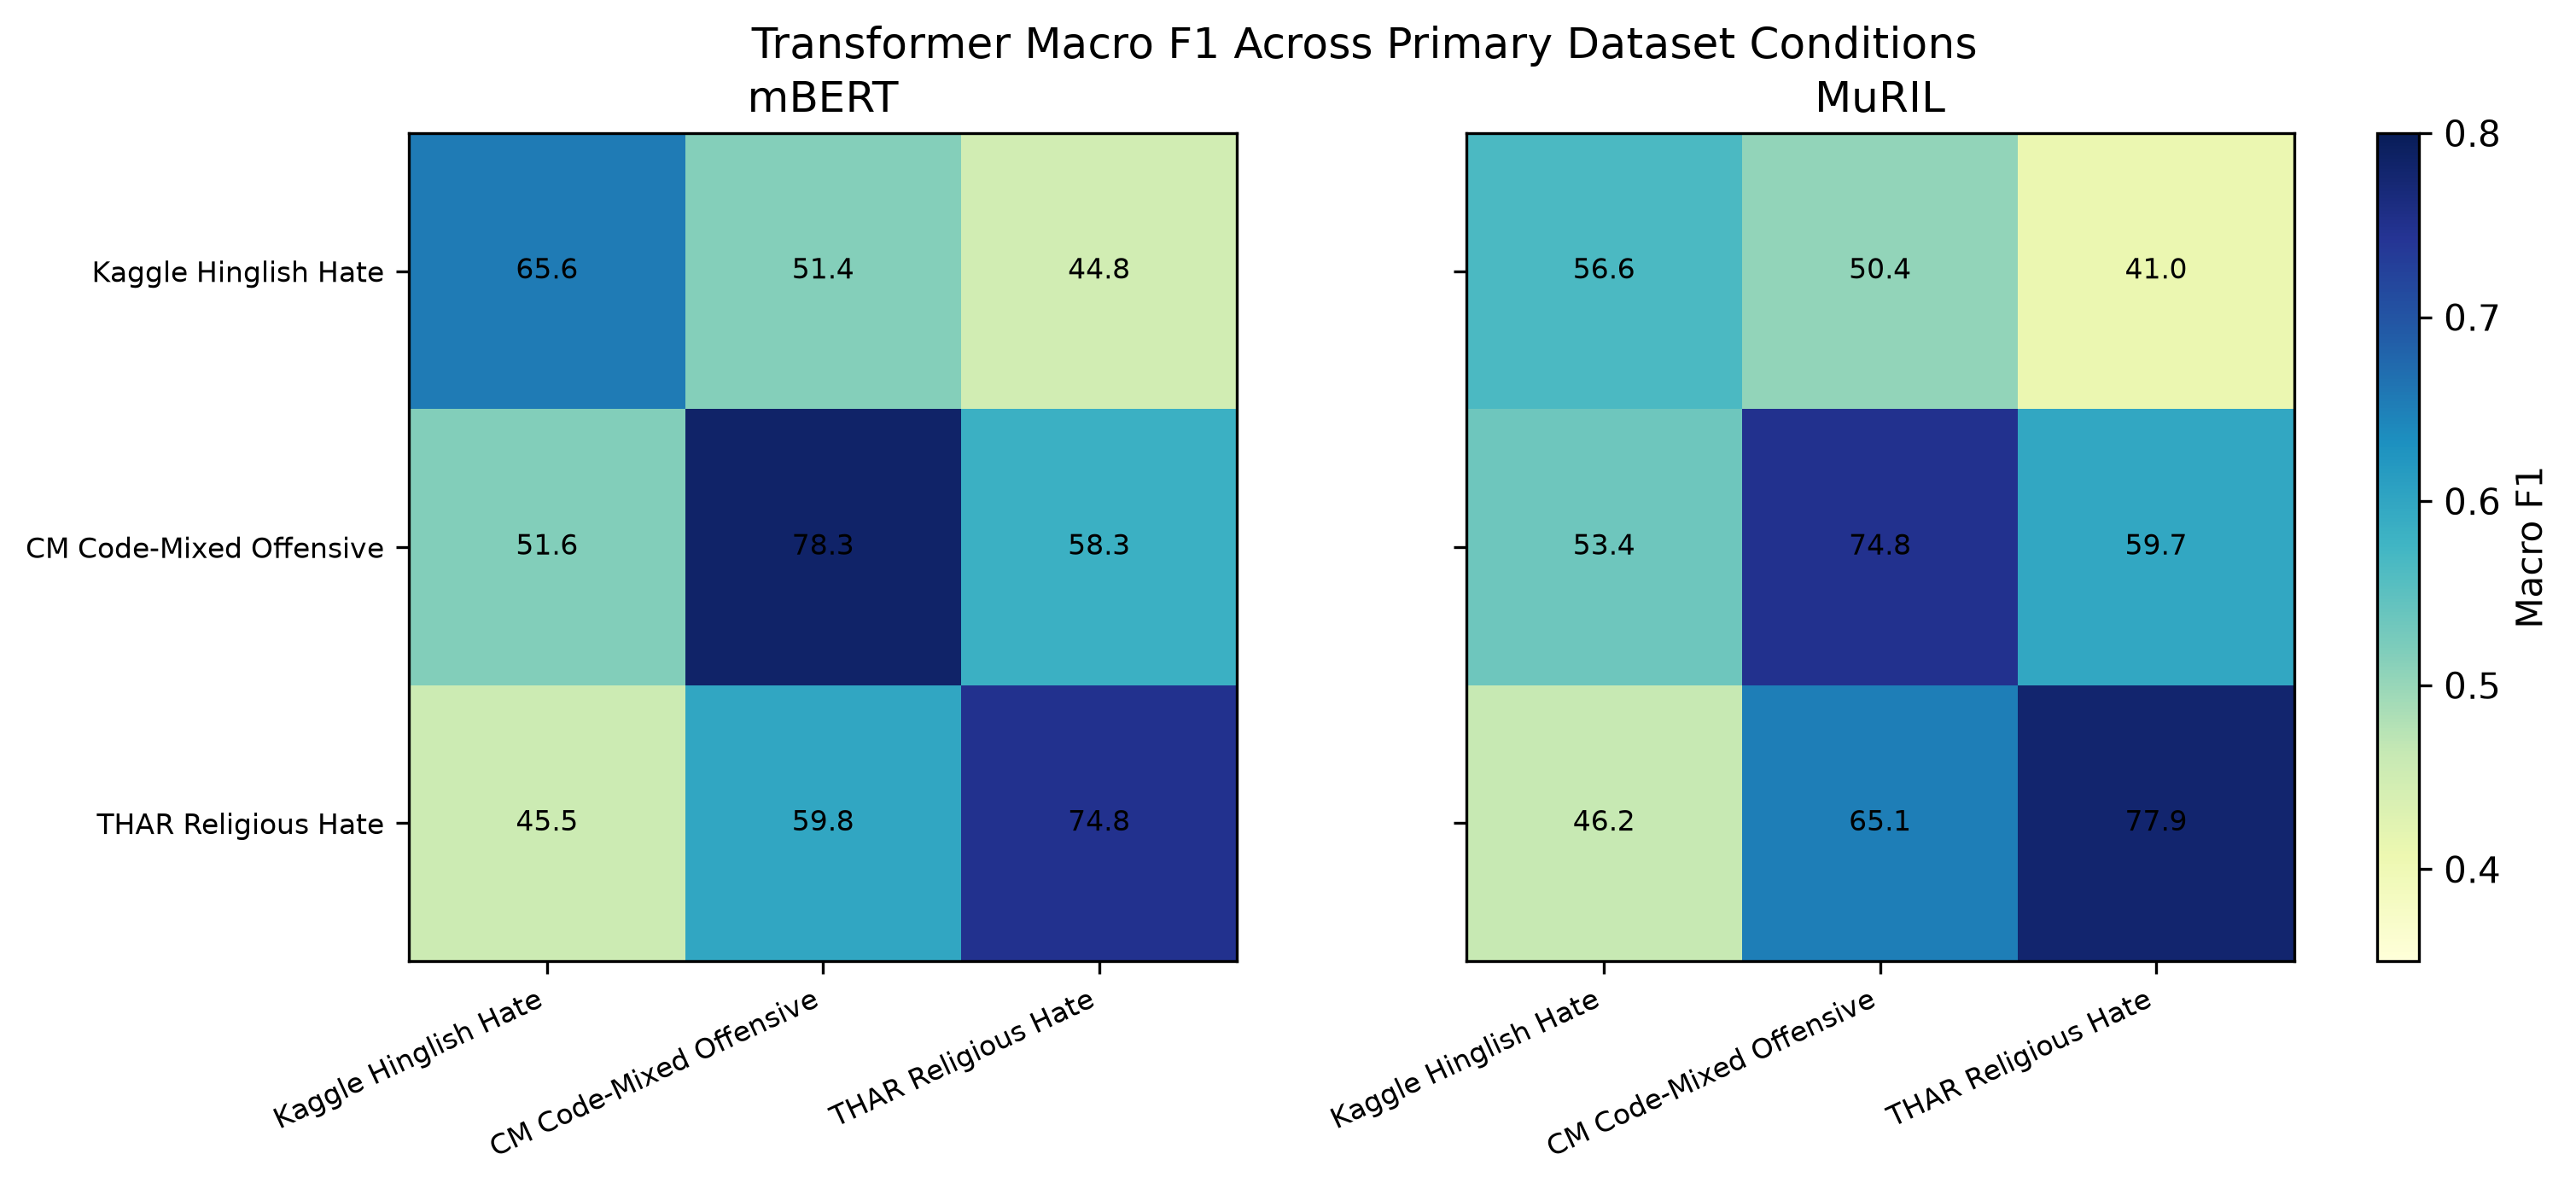
\includegraphics[width=0.85\textwidth]{transformer_primary_macro_f1_matrix.png}
\caption{Macro F1 for primary transformer train/test combinations.}
\label{fig:macro-matrix}
\end{figure}

These results already complicate the original model-comparison question. If only the Kaggle or CM matched setting is used, \mbert{} appears stronger. If only THAR is used, \muril{} appears stronger. The model ranking is therefore not stable across label definitions and domains.

\subsection{Cross-Dataset Transfer}

Cross-dataset transfer tests whether a model trained on one dataset can generalize to another. Table~\ref{tab:transfer} summarizes representative transfer conditions that changed the interpretation of the project.

\begin{table}[t]
\centering
\small
\begin{tabular}{l l l r r r}
\toprule
Train dataset & Test dataset & Model & Pos. recall & Pos. F1 & Macro F1 \\
\midrule
\datasetid{cm\_splits\_codemixed} & \datasetid{thar\_religion} & \mbert{} & 44.6 & 51.0 & 58.3 \\
\datasetid{cm\_splits\_codemixed} & \datasetid{thar\_religion} & \muril{} & 59.5 & 58.3 & 59.7 \\
\datasetid{thar\_religion} & \datasetid{cm\_splits\_codemixed} & \mbert{} & 40.1 & 45.0 & 59.8 \\
\datasetid{thar\_religion} & \datasetid{cm\_splits\_codemixed} & \muril{} & 53.1 & 54.4 & 65.1 \\
\datasetid{kaggle\_hinglish\_hate} & \datasetid{thar\_religion} & \mbert{} & 15.9 & 24.0 & 44.8 \\
\datasetid{kaggle\_hinglish\_hate} & \datasetid{thar\_religion} & \muril{} & 8.2 & 14.2 & 41.0 \\
\datasetid{thar\_religion} & \datasetid{kaggle\_hinglish\_hate} & \mbert{} & 20.6 & 25.5 & 45.5 \\
\datasetid{thar\_religion} & \datasetid{kaggle\_hinglish\_hate} & \muril{} & 23.3 & 27.7 & 46.2 \\
\bottomrule
\end{tabular}
\caption{Selected cross-dataset transfer results. Values are percentages.}
\label{tab:transfer}
\end{table}

\begin{figure}[t]
\centering
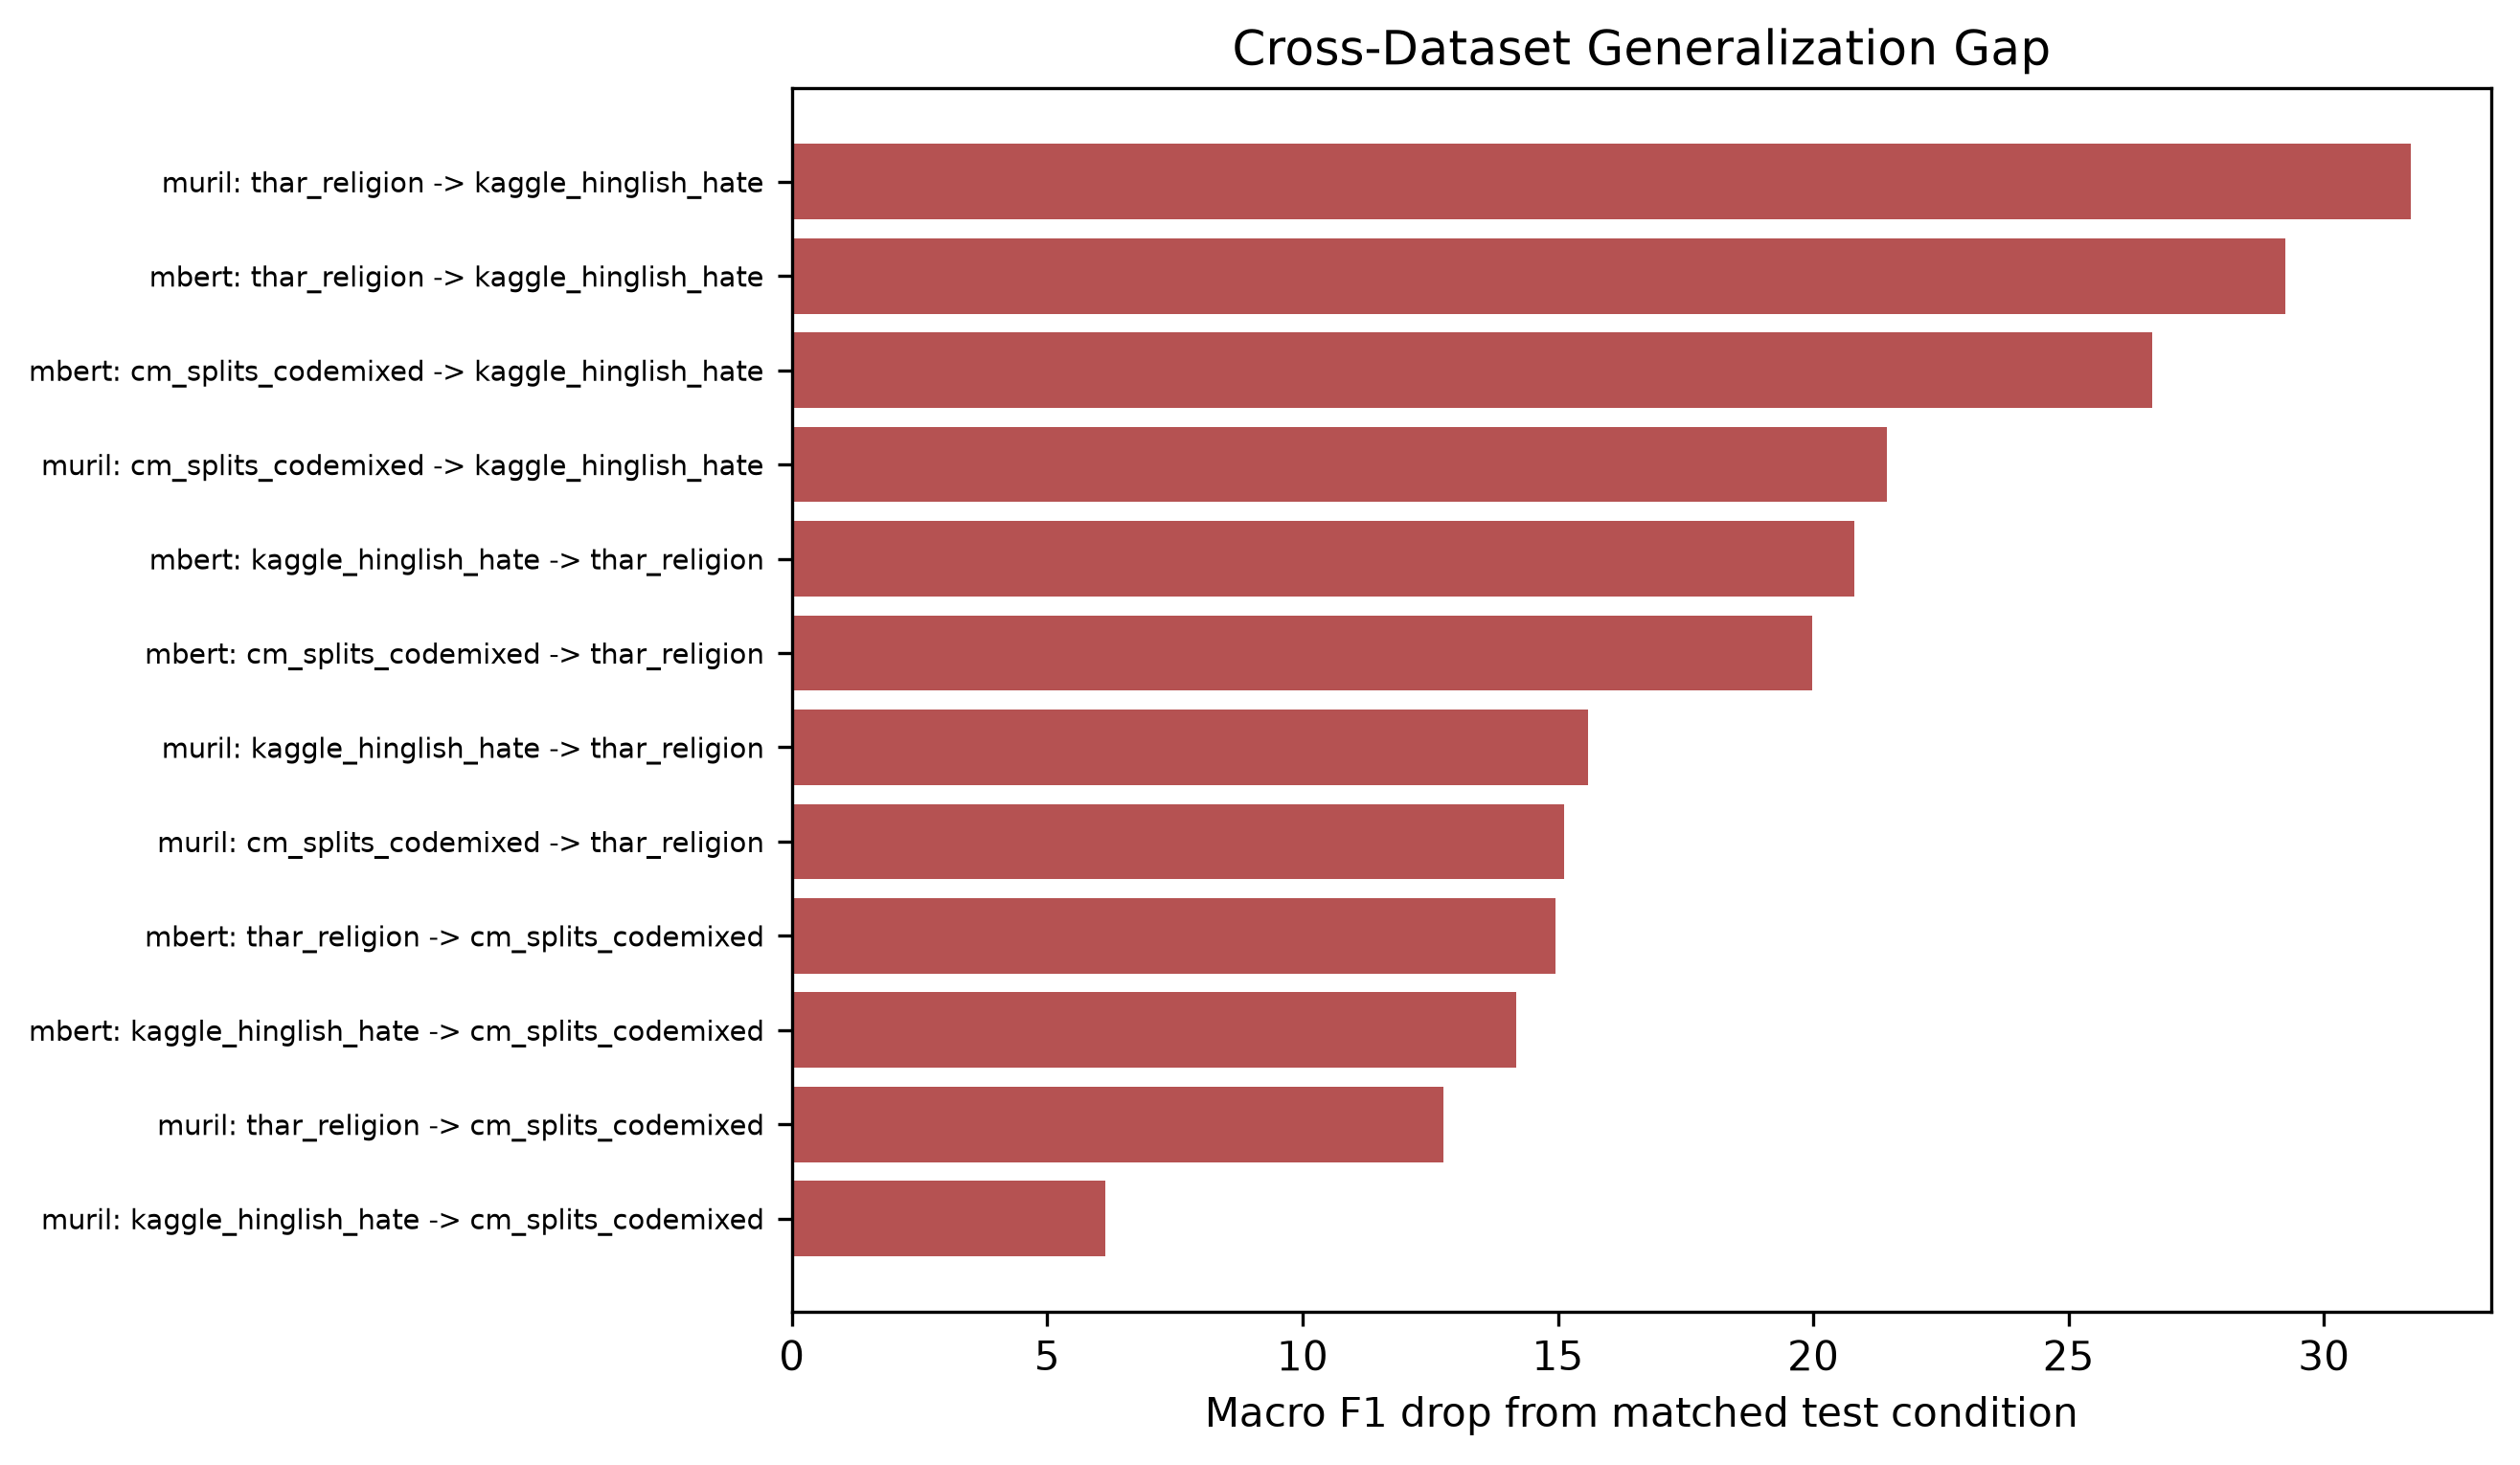
\includegraphics[width=0.9\textwidth]{transformer_generalization_gaps.png}
\caption{Generalization gaps between matched and cross-dataset evaluation.}
\label{fig:gaps}
\end{figure}

The strongest transfer pattern is that \muril{} improves THAR-related transfer, especially CM-to-THAR and THAR-to-CM. However, neither model transfers well between broad Hinglish hate and targeted religious hate. Kaggle-trained models are especially conservative on THAR, with very low positive recall, while THAR-trained models do not become general-purpose Hinglish hate detectors.

\subsection{Baselines}

Table~\ref{tab:baselines} compares the best transformer with the best TF-IDF baseline for selected settings. Transformers are strongest in matched conditions, but TF-IDF remains competitive and even wins in some transfer settings.

\begin{table}[t]
\centering
\small
\begin{tabularx}{\textwidth}{l l l r X r r}
\toprule
Train dataset & Test dataset & Best transformer & Trans. macro F1 & Best TF-IDF & TF-IDF macro F1 & Delta \\
\midrule
\datasetid{cm\_splits\_codemixed} & \datasetid{cm\_splits\_codemixed} & \mbert{} & 78.3 & Logistic & 77.6 & 0.7 \\
\datasetid{kaggle\_hinglish\_hate} & \datasetid{kaggle\_hinglish\_hate} & \mbert{} & 65.6 & Logistic & 61.4 & 4.1 \\
\datasetid{thar\_religion} & \datasetid{thar\_religion} & \muril{} & 77.9 & Logistic & 70.6 & 7.3 \\
\datasetid{kaggle\_hinglish\_hate} & \datasetid{thar\_religion} & \mbert{} & 44.8 & Logistic & 49.9 & -5.2 \\
\datasetid{thar\_religion} & \datasetid{kaggle\_hinglish\_hate} & \muril{} & 46.2 & Logistic & 51.0 & -4.9 \\
\bottomrule
\end{tabularx}
\caption{Best transformer versus best TF-IDF baseline. Delta is transformer macro F1 minus TF-IDF macro F1, in percentage points.}
\label{tab:baselines}
\end{table}

This matters for the paper's interpretation. A strong transformer result should not be reported without a lexical baseline, because dataset-specific keywords and repeated expressions can carry much of the signal.

\section{Error Analysis}

The error analysis focuses on false negatives, disagreement cases, script composition, and qualitative reasons for failure. Table~\ref{tab:fn} reports selected false-negative rates. A false negative is a positive example predicted as negative.

\begin{table}[t]
\centering
\small
\begin{tabular}{l l r r}
\toprule
Train dataset & Test dataset & \mbert{} FN rate & \muril{} FN rate \\
\midrule
\datasetid{kaggle\_hinglish\_hate} & \datasetid{kaggle\_hinglish\_hate} & 61.4 & 77.7 \\
\datasetid{cm\_splits\_codemixed} & \datasetid{cm\_splits\_codemixed} & 31.3 & 44.9 \\
\datasetid{thar\_religion} & \datasetid{thar\_religion} & 22.3 & 19.7 \\
\datasetid{kaggle\_hinglish\_hate} & \datasetid{thar\_religion} & 84.1 & 91.8 \\
\datasetid{thar\_religion} & \datasetid{kaggle\_hinglish\_hate} & 79.4 & 76.7 \\
\datasetid{thar\_religion} & \datasetid{cm\_splits\_codemixed} & 59.9 & 46.9 \\
\bottomrule
\end{tabular}
\caption{Selected false-negative rates. Values are percentages.}
\label{tab:fn}
\end{table}

\begin{figure}[t]
\centering
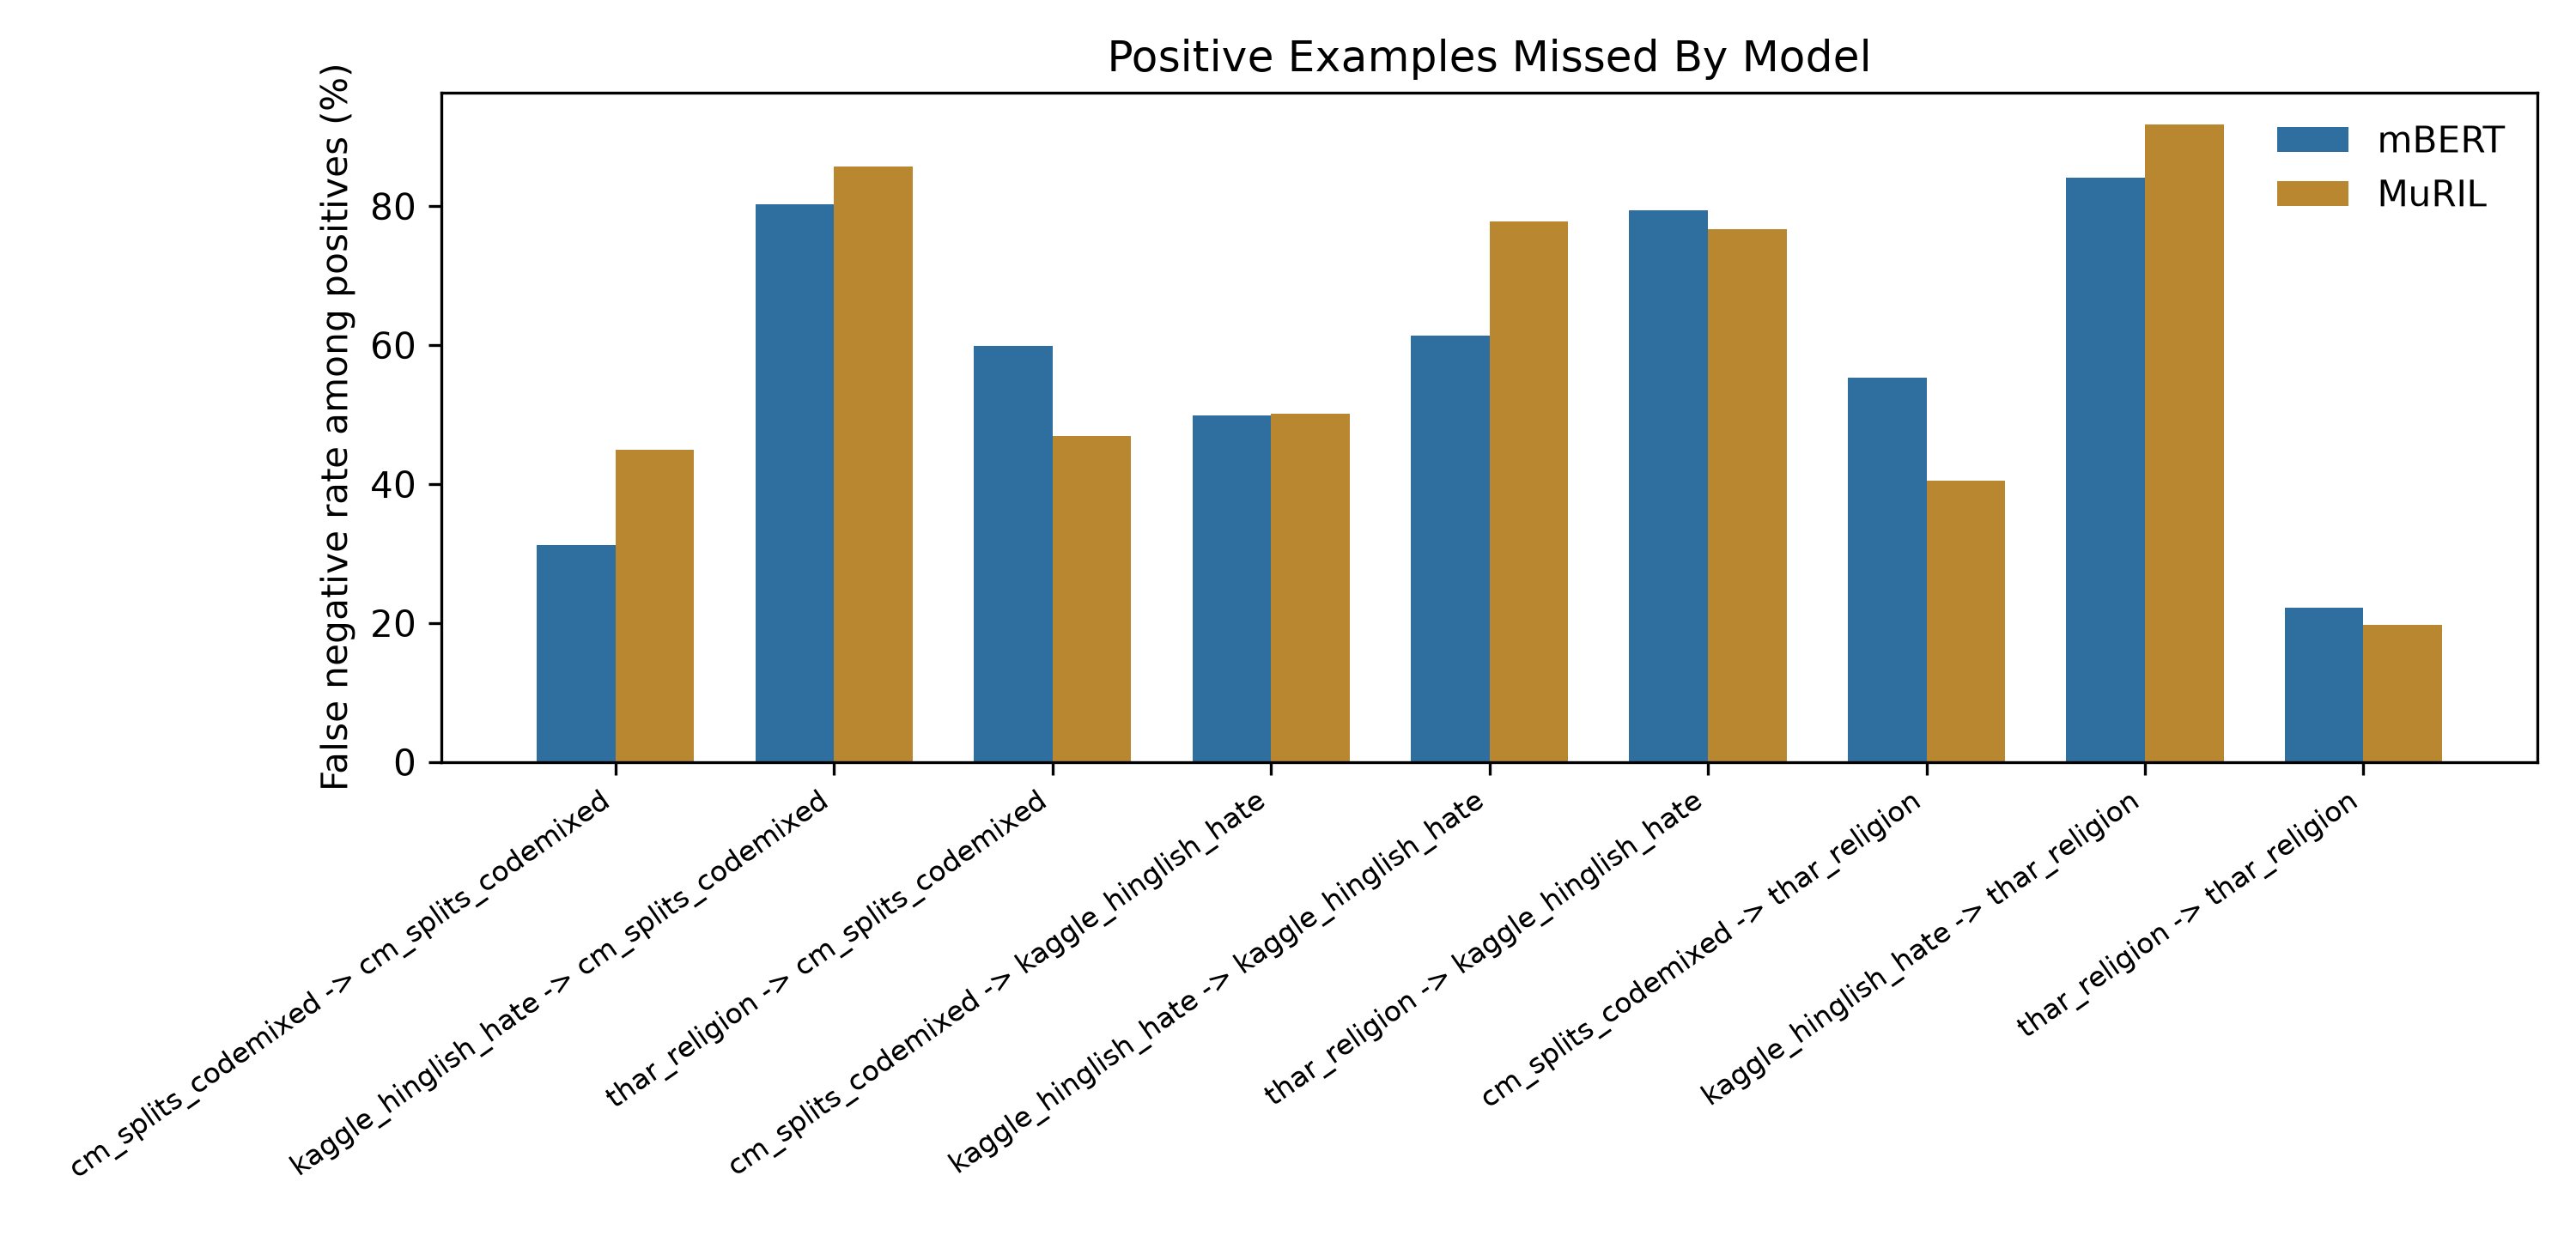
\includegraphics[width=0.9\textwidth]{false_negative_rates.png}
\caption{False-negative rates across primary train/test conditions.}
\label{fig:fn}
\end{figure}

The false-negative analysis supports the same conditional model story. \mbert{} misses fewer positives on matched Kaggle and CM, while \muril{} misses fewer positives on matched THAR and THAR-to-CM transfer. Feature-level analysis also suggests that script and target domain matter. Across error rows, Devanagari-only positives were missed more often than Latin-only positives, and \muril{} had a lower false-negative rate than \mbert{} on Devanagari-only rows in the current error analysis.

A first-pass manual coding of sampled errors found that the most common reason was cross-dataset label mismatch. Other recurring reasons included generic profanity or abuse, target-group or religion cues, political context or slogans, short/contextless text, and script complexity. This qualitative result explains why cross-dataset transfer is difficult: many failures are not simply model mistakes but collisions between different annotation policies and social contexts.

\section{Discussion}

The current results do not support a simple claim that \mbert{} or \muril{} is better in general. Instead, the project finds that model choice interacts with dataset situation.

\mbert{} appears stronger when the evaluation condition is mostly Latin-script Hinglish or code-mixed offensive text, as in the matched Kaggle and CM conditions. One possible explanation is that \mbert{} handles the Latin-script and English-like surface form of Romanized Hinglish well enough to learn dataset-specific lexical cues. This is consistent with its stronger positive recall on Kaggle and CM matched tests.

\muril{} appears stronger when the evaluation condition includes targeted Indian-context religious hate or more Devanagari/mixed-script text, as in THAR. This is consistent with \muril{}'s design goal of improving representations for Indian languages and transliteration, although the present experiments do not prove the mechanism causally. The safer interpretation is that \muril{} performs better in THAR-related conditions under the current setup.

The cross-dataset results are the most important part of the project. Each primary test dataset is best served by a model trained on the same dataset. When models move across datasets, macro F1 and positive recall often drop sharply. This shows that the datasets are not interchangeable, even though all are related to Hinglish, Hindi-English code-mixing, hate speech, or offensive language.

\section{Limitations}

This draft has several limitations. First, the datasets use different positive-label definitions. Hate, offensive language, and targeted anti-religion hate are related but not identical categories. Second, platform differences are large: Twitter/X and YouTube comments have different styles, contexts, and audience behavior. Third, the current project uses public datasets rather than a newly annotated, India-focused evaluation set with a single unified annotation scheme. Fourth, the CM dataset license and citation details require final verification before publication. Fifth, the 79-row diagnostic probe is excluded from primary conclusions because its provenance is uncertain.

The project also reviewed Indo-HateSpeech as a possible fourth dataset. It is accessible and citable, but the local audit found many short, duplicate, or potentially ambiguous examples concentrated in Instagram comments from a limited set of post IDs. The current decision is not to add it to the primary experiment set before mixed training, although it may be useful later as a secondary robustness test if filtered and reported carefully.

\section{Conclusion}

This project began as a direct comparison between \mbert{} and \muril{} for Hinglish hate speech detection. The evidence so far suggests a more useful conclusion: model superiority is conditional on dataset situation. \mbert{} is stronger on matched Latin-script Hinglish and code-mixed offensive datasets, while \muril{} is stronger on targeted religious hate and some THAR-related transfer settings. Cross-dataset evaluation reveals large generalization gaps, and TF-IDF baselines show that lexical cues remain strong.

The final paper should therefore argue that evaluation design is central to Hinglish hate speech detection. A single in-domain score can hide transfer failures, while cross-dataset testing reveals how model behavior changes with script, platform, target, and label definition.

\section{Future Work}

The next stage is mixed-dataset training. Models should be trained on combinations such as Kaggle+CM, Kaggle+THAR, CM+THAR, and Kaggle+CM+THAR, then tested separately on each dataset. This will test whether broader training improves robustness or simply blends incompatible label definitions. Future work should also include threshold tuning, stronger documentation of dataset licenses, a more formal manual error analysis sample, and possibly a small India-focused evaluation set with clear annotation guidelines.

\bibliographystyle{plainnat}
\bibliography{references}

\end{document}
